\cohead{\Large\textbf{Funktionen}}
\subsection[Funktionen]{Funktionen im SELECT-Statement}\label{funktionen}
Öffne die Datenbank \texttt{schule.db} mit dem Datenbank-Browser oder sqlite3.exe.\\
SQL bietet einige einfache Funktionen an, die man innerhalb des SELECT-Statements verwenden kann:
\begin{tcolorbox}[title=Funktionen in SQL]
	\lstinline!SELECT FUNKTIONSNAME(name_attribut) FROM name_tabelle (WHERE bedingungen);!
\end{tcolorbox}
\begin{itemize}
	\item \lstinline!COUNT!	Anzahl der Werte zählen
	\item \lstinline!MAX!	Maximalwert bestimmen
	\item \lstinline!MIN!	Minimalwert bestimmen
	\item \lstinline!AVG!	Durchschnittswert bestimmen
	\item \lstinline!SUM!	Werte summieren
\end{itemize}

Offensichtlich kann man bis auf die COUNT-Funktion als Argument sinnvoll nur Attribute mit einer Zahl als Datentyp anwenden.\\
Verwendung als SQL-Statements:
\begin{itemize}
	\item \lstinline!SELECT COUNT(schuelerNR) FROM schueler;!\\
	Gibt die Anzahl der Einträge in der Tabelle schueler zurück.
	\item \lstinline!SELECT COUNT(schuelerNR) FROM schueler WHERE plz=70806;!\\
	Gibt die Anzahl der Schüler zurück, die die plz 70806 haben.
	\item \lstinline!SELECT COUNT(lehrerNR) FROM lehrer WHERE nachname LIKE 'S%';!\\
	Gibt die Anzahl an Lehrern zurück, deren Nachname mit einem S beginnt.
\end{itemize}
Mit dem Zusatz \lstinline!GROUP BY! kann man Datensätze, die in einem Attribut übereinstimmen, zusammenfassen:
\begin{itemize}
	\item \lstinline!SELECT COUNT(lehrerNR) FROM unterrichtet;!
	Gibt die Anzahl der Einträge in der Tabelle \lstinline!unterrichtet! zurück.
	\item \lstinline!SELECT klasseNR, COUNT(lehrerNR) FROM unterrichtet GROUP BY klasseNR;!
	Gibt die Anzahl verschiedener Lehrer (eigentlich die Anzahl von Einträgen pro Klasse) für jede Klasse bzw. \lstinline!klasseNR! zurück.
\end{itemize}

\begin{Exercise}[title={Bearbeite folgende Aufgaben}, label=Funktionen]
	\begin{enumerate}
		\item Erstelle ein zur Datenbank passendes ERM. Tipp: \lstinline!.schema! könnte hilfreich sein.
		\item Wie viele verschiedene Lehrer unterrichten an der Schule?
		\item Wie viele Schüler kommen aus einer Stadt, deren PLZ mit einer 7 beginnt?
		\item Wie viele Lehrer sind den einzelnen Abteilungen jeweils zugeordnet?
	\end{enumerate}
\end{Exercise}
%%%%%%%%%%%%%%%%%%%%%%%%%%%%%%%%%%%%%%%%%
\begin{Answer}[ref=Funktionen]
	\begin{enumerate}
		\item Erstelle ein zur Datenbank passendes ERM. Tipp: \lstinline!.schema! könnte hilfreich sein.\\
		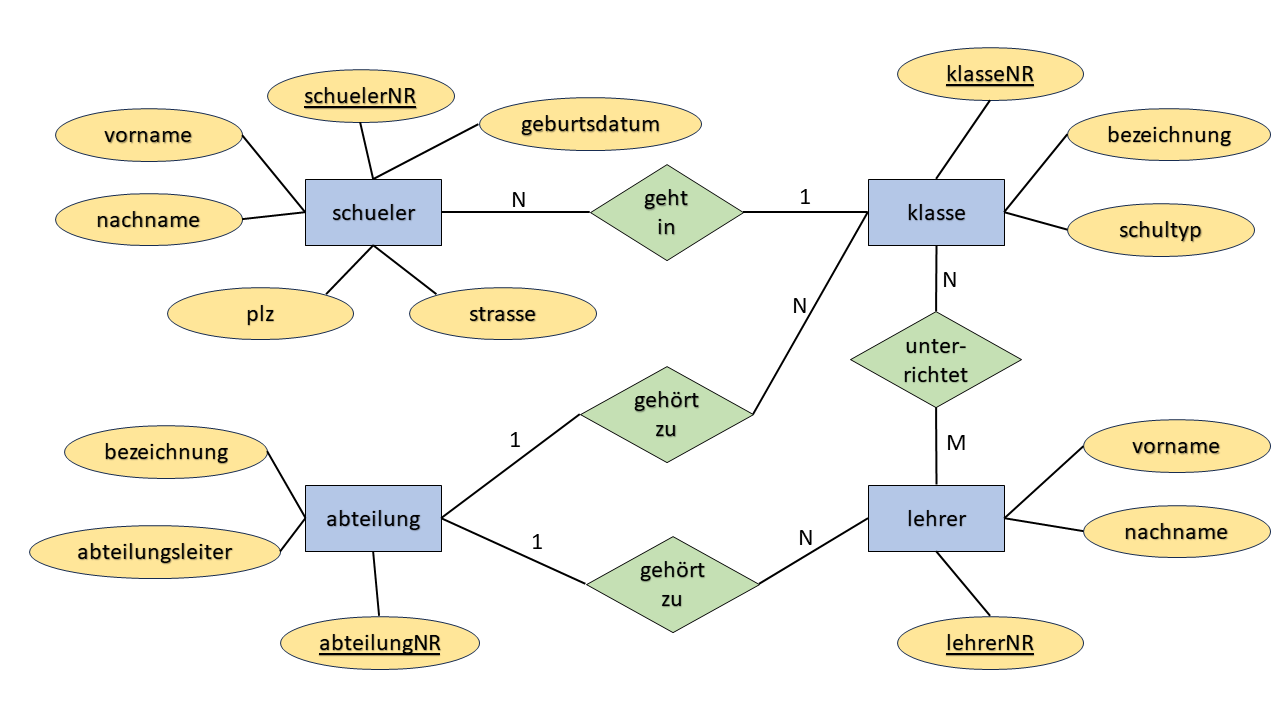
\includegraphics[width=\linewidth]{\pics/schuleDB.png}
		\item Wie viele verschiedene Lehrer unterrichten an der Schule?\\
		\lstinline!SELECT COUNT(lehrerNR) FROM lehrer;!\\
		Es sind 17 Lehrer.
		\item Wie viele Schüler kommen aus einer Stadt, deren PLZ mit einer 7 beginnt?\\
		\lstinline!SELECT COUNT(schuelerNR) FROM schueler WHERE plz between 70000 AND 79999;!\\
		Es sind 142 Schüler.
		\item Wie viele Lehrer sind den einzelnen Abteilungen jeweils zugeordnet?\\
		\lstinline!SELECT abteilungNR, COUNT(lehrerNR) FROM lehrer_abteilung GROUP BY abteilungNR;!\\
		\begin{lstlisting}
			3|6
			6|7
			8|3\end{lstlisting}
		\lstinline!SELECT abteilungNR, bezeichnung FROM abteilung;!\\
		\begin{lstlisting}
			3|WG
			6|Berufskolleg
			8|Berufsschule\end{lstlisting}
		Das bedeutet also, dass im WG 6 Lehrer, im Berufskolleg 7 Lehrer und in der Berufsschule 3 Lehrer unterrichten.
	\end{enumerate}
\end{Answer}